\documentclass[tikz,border=12pt]{standalone}
% Shared visual language for standalone EMT block diagrams.
\usepackage{amsmath}
\usetikzlibrary{arrows.meta,backgrounds,calc,fit,positioning}

\tikzset{
    emt diagram/.style = {>={Stealth[length=2.4mm]}},
    line/.style        = {semithick, rounded corners=6pt},
    block/.style       = {draw, semithick, fill=white,
                          minimum height=1cm, minimum width=2.3cm},
    hblock/.style      = {block, minimum width=2.24cm, minimum height=1.3cm},
    vblock/.style      = {block, minimum width=1.3cm, minimum height=2.24cm},
    sum/.style         = {draw, semithick, fill=white, circle,
                          inner sep=2.6pt},
    signal/.style      = {circle, fill, inner sep=1.4pt,
                          label distance=3pt},
    sig/.style         = {font=\small},
    pm/.style          = {font=\scriptsize},
    wire jump/.style   = {line,
                          preaction={draw=white, line width=3pt,
                                     line cap=round}},
    enclosure/.style   = {draw, dashed, semithick, rounded corners=4pt},
    operator enclosure/.style = {enclosure, inner xsep=7mm, inner ysep=6mm}
}


\begin{document}
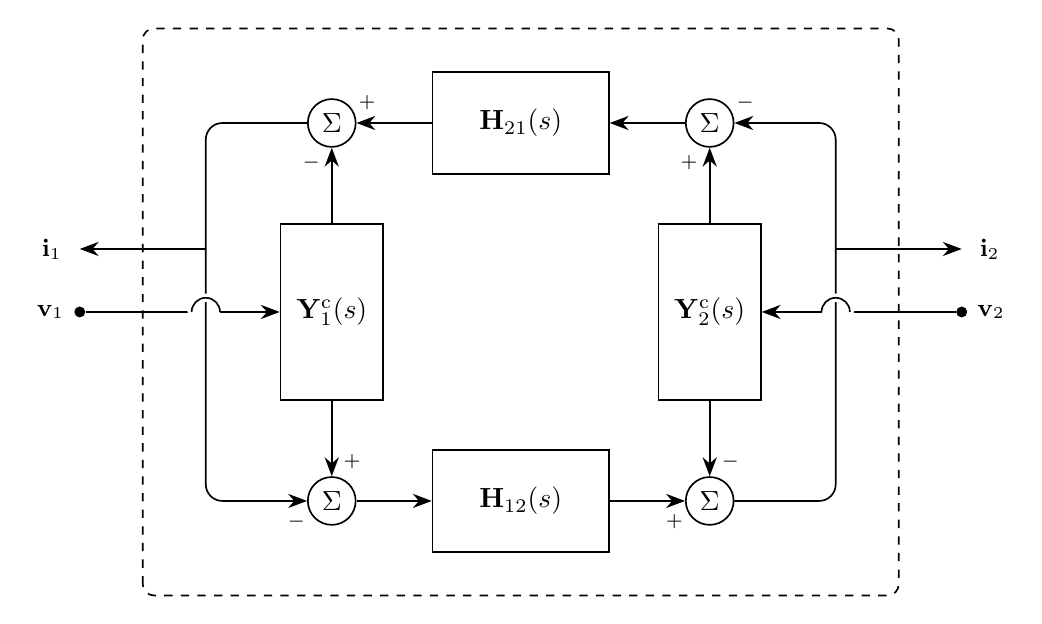
\begin{tikzpicture}[emt diagram]

% ================= Terminal 1 (left column) =================
\node[sum]   (kcl1)  at (-2.4,  2.4) {$\Sigma$};
\node[vblock] (Yc1)  at (-2.4,  0.0) {$\mathbf{Y}^{\mathrm{c}}_1(s)$};
\node[sum]   (wave1) at (-2.4, -2.4) {$\Sigma$};

\node[signal, label={[sig]left:$\mathbf{v}_1$}] (v1) at (-5.6, 0) {};

\draw[->, line] (Yc1.north) -- (kcl1);
\draw[->, line] (Yc1.south) -- (wave1);
\draw[->, line] (kcl1.west) -- (-4.0, 2.4)
                                -- (-4.0, -2.4) -- (wave1);
\coordinate (i1port) at (-5.6, 0.8);
\draw[->, line] (-4.0, 0.8) -- (i1port);
\node[sig, left=3pt of i1port] {$\mathbf{i}_1$};

% Voltage lead crosses over the continuous current path.
\draw[line] (v1) -- (-4.18, 0);
\draw[wire jump] (-4.18, 0)
    arc[start angle=180, end angle=0, radius=0.18];
\draw[->, line] (-3.82, 0) -- (Yc1.west);

% ================= Terminal 2 (right column) =================
\node[sum]   (wave2) at (2.4,  2.4) {$\Sigma$};
\node[vblock] (Yc2)  at (2.4,  0.0) {$\mathbf{Y}^{\mathrm{c}}_2(s)$};
\node[sum]   (kcl2)  at (2.4, -2.4) {$\Sigma$};

\node[signal, label={[sig]right:$\mathbf{v}_2$}] (v2) at (5.6, 0) {};

\draw[->, line] (Yc2.north) -- (wave2);
\draw[->, line] (Yc2.south) -- (kcl2);
\draw[->, line] (kcl2.east) -- (4.0, -2.4)
                               -- (4.0, 2.4) -- (wave2);
\coordinate (i2port) at (5.6, 0.8);
\draw[->, line] (4.0, 0.8) -- (i2port);
\node[sig, right=3pt of i2port] {$\mathbf{i}_2$};

% Voltage lead crosses over the continuous current path.
\draw[line] (v2) -- (4.18, 0);
\draw[wire jump] (4.18, 0)
    arc[start angle=0, end angle=180, radius=0.18];
\draw[->, line] (3.82, 0) -- (Yc2.east);

% ================= Propagation channels (straight rows) =================
% 1 -> 2 (lower row, left to right)
\node[hblock] (H12) at (0, -2.4) {$\mathbf{H}_{12}(s)$};
\draw[->, line] (wave1.east) -- (H12.west);
\draw[->, line] (H12.east) -- (kcl2.west);

% 2 -> 1 (upper row, right to left)
\node[hblock] (H21) at (0,  2.4) {$\mathbf{H}_{21}(s)$};
\draw[->, line] (wave2.west) -- (H21.east);
\draw[->, line] (H21.west) -- (kcl1.east);

% ================= Summation signs =================
\node[pm] at ($(kcl1)+(-0.26,-0.50)$) {$-$};   % Yc1 v1 subtracts
\node[pm] at ($(kcl1)+( 0.45, 0.26)$) {$+$};   % incident current adds
\node[pm] at ($(wave1)+(0.26, 0.50)$) {$+$};   % Yc1 v1
\node[pm] at ($(wave1)+(-0.45,-0.26)$) {$-$};  % i1
\node[pm] at ($(kcl2)+( 0.26, 0.50)$) {$-$};   % Yc2 v2 subtracts
\node[pm] at ($(kcl2)+(-0.45,-0.26)$) {$+$};   % incident current adds
\node[pm] at ($(wave2)+(-0.26,-0.50)$) {$+$};  % Yc2 v2
\node[pm] at ($(wave2)+( 0.45, 0.26)$) {$-$};  % i2

% ================= Model enclosure =================
\draw[enclosure] (-4.8, -3.6) rectangle (4.8, 3.6);

\end{tikzpicture}
\end{document}
